\chapter{Perfis de carga e resposta dos detectores em dados reais}\label{demonstracao-experimental-das-tecnicas-de-ml}
\section{Forma intradiária da carga}
A extração exploratória recuperou perfis de 12 UCs com cobertura de pelo menos 80\% e partições intervalares disponíveis. Para cada UC, dividiu-se a mediana de energia de cada hora pela soma das 24 medianas. Cada curva da Figura~\ref{perfis-reais} soma 100\%. Um pico indica concentração horária relativa. A amplitude absoluta deve ser consultada em kWh. A seleção por disponibilidade limita a interpretação da frequência desses formatos no parque.

\begin{figure}[htbp]\centering\caption{Distribuição horária da energia em 12 perfis medidos}\label{perfis-reais}
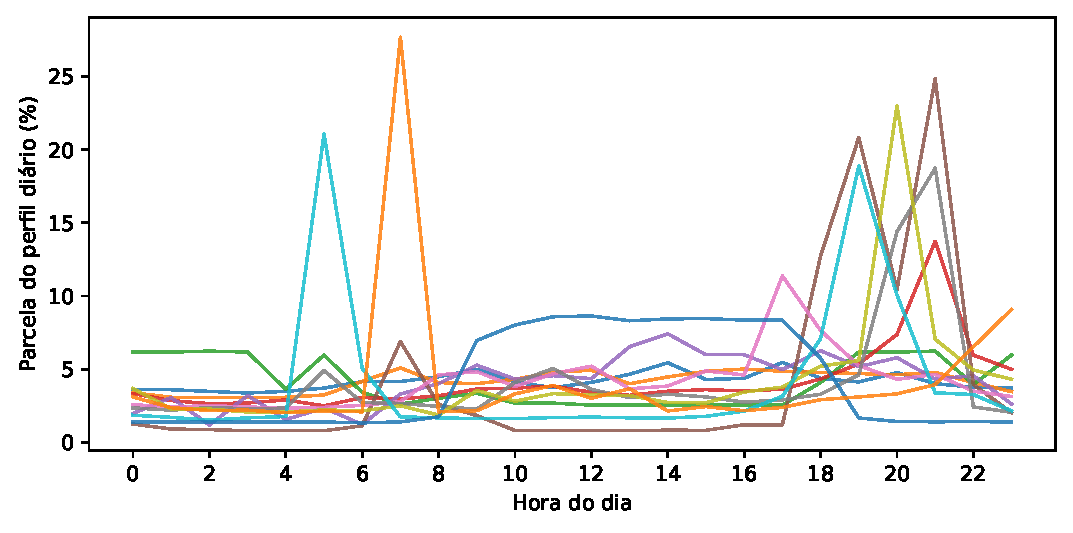
\includegraphics[width=.90\linewidth]{figuras/perfis_reais.pdf}
\par\small Fonte: elaboração própria a partir das medianas horárias de memória de massa.
\end{figure}
\section{Concordância entre detectores}
O Isolation Forest separa observações por partições aleatórias, atribuindo maior raridade àquelas isoladas por caminhos curtos \autocite{liu2008}. O LOF compara a densidade local de uma observação à de seus vizinhos \autocite{breunig2000}; por isso, diferenças de escala e empates requerem controle. ECOD e COPOD empregam informações de caudas e distribuições empíricas \autocite{li2022ecod,li2020copod}; HBOS utiliza histogramas por atributo \autocite{goldstein2012hbos}, todos alinhados à formulação do ecossistema PyOD \autocite{zhao2019pyod}. O resíduo da PCA quantifica a distância entre o vetor e sua reconstrução no subespaço retido. Os detectores não são, a priori, independentes. A comparação de correlações e a retirada de componentes no ensaio OOT, descritas nos resultados, permitem avaliar a diferença entre suas ordenações sem pressupor ganho de precisão.


A Figura~\ref{det-real} reúne os escores pareados de IF e LOF para as 65.686 UCs do corte de 19/11. Cada célula conta as unidades que receberam aquele par de escores. As células afastadas da diagonal mostram onde uma mesma UC recebeu avaliações diferentes de raridade global e local. A ablação da Tabela~\ref{ablacao} quantifica o efeito dessa diferença na lista de inspeção. A confirmação de uma irregularidade requer desfecho independente.

\begin{figure}[htbp]\centering\caption{Escores individuais de IF e LOF na inferência OOT}\label{det-real}
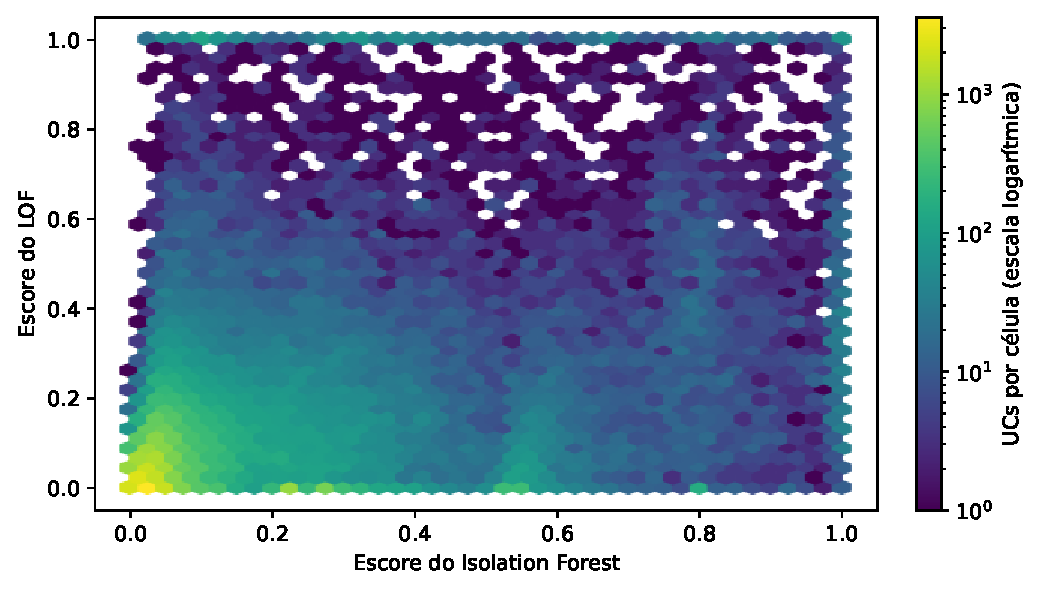
\includegraphics[width=.88\linewidth]{figuras/if_lof_oot.pdf}
\par\small Fonte: elaboração própria a partir dos escores congelados do corte de 19/11/2026.
\end{figure}

As respostas complementares de isolamento, densidade local e contextualização também são ilustradas em um experimento sintético controlado, apresentado no Apêndice~\ref{ap:demonstracoes}. Esse ensaio permite examinar mecanismos sob condições conhecidas, sem substituir os resultados AMI reais nem estimar a frequência de irregularidades na população.
